%--------------------------------------------------------------
%--------------------------------------------------------------
% Section 2 : MPTK for Windows
%--------------------------------------------------------------
%--------------------------------------------------------------
\chapter{MPTK for Windows \label{MptkForWin}}

%--------------------------------------------------------------
% Section 2.1 : Downloading MPTK
%--------------------------------------------------------------
\section{Downloading MPTK}

The latest version of MPTK is available at (https://gforge.inria.fr/frs/?group\_id=36). Depending on the processor architecture of 
your computer, you will have to download either the 32 bits package or the 64 bits package:
\begin{my_itemize}
	\item For Windows 32 bits : ``MPTK-binary-v.v.v-i386-Windows.exe''
	\item For Windows 64 bits : ``MPTK-binary-v.v.v-x86\_64-Windows.exe''
\end{my_itemize}

\noindent \emph{\underline{Hint :} To find the processor architecture of your computer:}
\begin{my_itemize}
	\item \emph{Open a terminal command using :}
	\begin{my_itemize}
		\item \emph{Start $\mapsto$ All Programs $\mapsto$ Accessories $\mapsto$ Command Prompt}
	\end{my_itemize}
	\item \emph{Use the following command : \textcolor[rgb]{0.4,0.4,0.4}{echo \%PROCESSOR\_ARCHITECTURE\%}}
	\begin{my_itemize}
		\item \emph{If the answer is ``x86'' then your OS is 32 bits}
		\item \emph{If the answer is ``AMD64'' then your OS is 64 bits}
	\end{my_itemize}
\end{my_itemize}

%--------------------------------------------------------------
% Section 2.2 : Installing MPTK
%--------------------------------------------------------------
\section{Installing MPTK}

When double clicking the executable ``MPTK-binary-v.v.v.-(i386/x86\_64)-Windows.exe'':
\begin{enumerate}
	\item Accept the terms of the licence agreement
	\item Select the path folder where to install MPTK (we'll call it  \emph{``path\_to\_MPTK''})
	\begin{my_itemize}
		\item We suggest to use the default folder : ``C:\textbackslash Program Files\textbackslash MPTK''
	\end{my_itemize}
	\item Finish the installation
\end{enumerate}	

\begin{figure}[H]
	\begin{minipage}[t]{.4\linewidth}
   	 	\begin{center}
			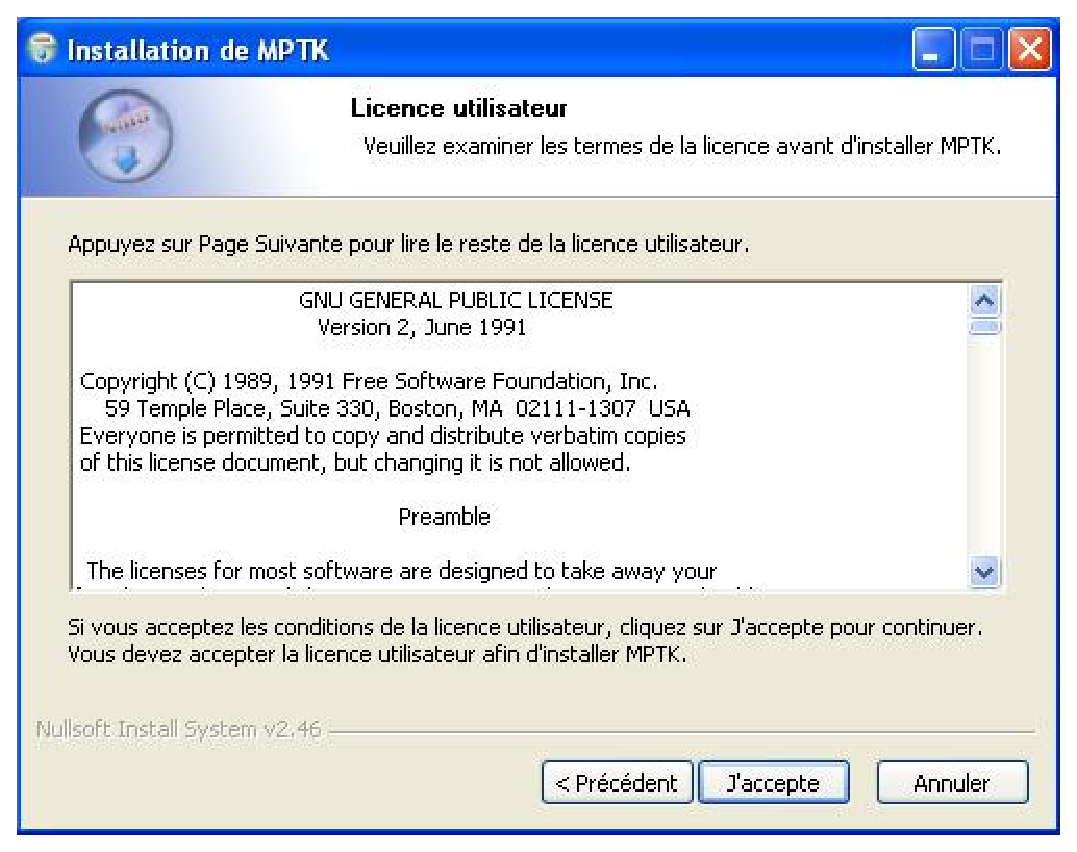
\includegraphics[width = 7cm, height=5cm]{Images/WindowsLicence.eps}
			\textit{\caption{\label{WindowsLicence} Licence agreement}}
		\end{center}
	\end{minipage}
	\hfill
	\begin{minipage}[t]{.4\linewidth}
		\begin{center}
			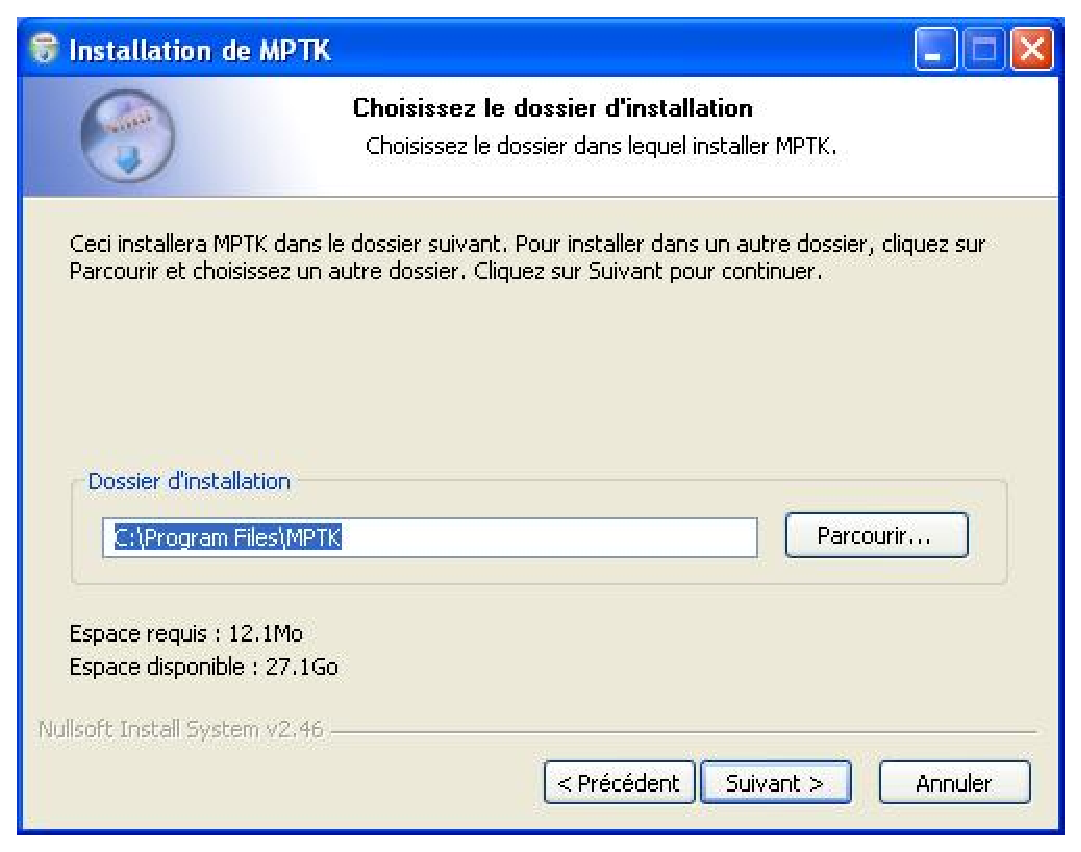
\includegraphics[width = 7cm, height=5cm]{Images/PathSelection.eps}
			\textit{\caption{\label{PathSelection}Path folder selection}}
		\end{center}
	\end{minipage}
\end{figure}

%--------------------------------------------------------------
% Section 2.3 : Configuring the path
%--------------------------------------------------------------
\section{Configuring the path}

An environment variable called \begin{footnotesize}MPTK\_CONFIG\_FILENAME\end{footnotesize} needs to be set, either temporarily, or permanently, 
with the path of the ``path.xml'' file located in the \emph{``path\_to\_MPTK/mptk''} directory. This file defines the environment 
paths that MPTK needs to work correctly.


% Section 2.3.1 : Temporary path configuration

\subsection{Temporary path configuration}

Here is the way to temporarily configure the \begin{footnotesize}MPTK\_CONFIG\_FILENAME\end{footnotesize} environment variable. 
\textbf{Warning} : This is a temporary setting and it needs to be done at each reset of the computer.

\begin{my_itemize}
	\item Open a terminal command using :
	\begin{my_itemize}
		\item Start $\mapsto$ All Programs $\mapsto$ Accessories $\mapsto$ Command Prompt
	\end{my_itemize}
	\item Use the command : \textcolor[rgb]{0.4,0.4,0.4}{\emph{set \begin{footnotesize}MPTK\_CONFIG\_FILENAME\end{footnotesize} = path\_to\_MPTK/mptk/path.xml}}
\end{my_itemize}

\begin{figure}[H]
   	 \begin{center}
		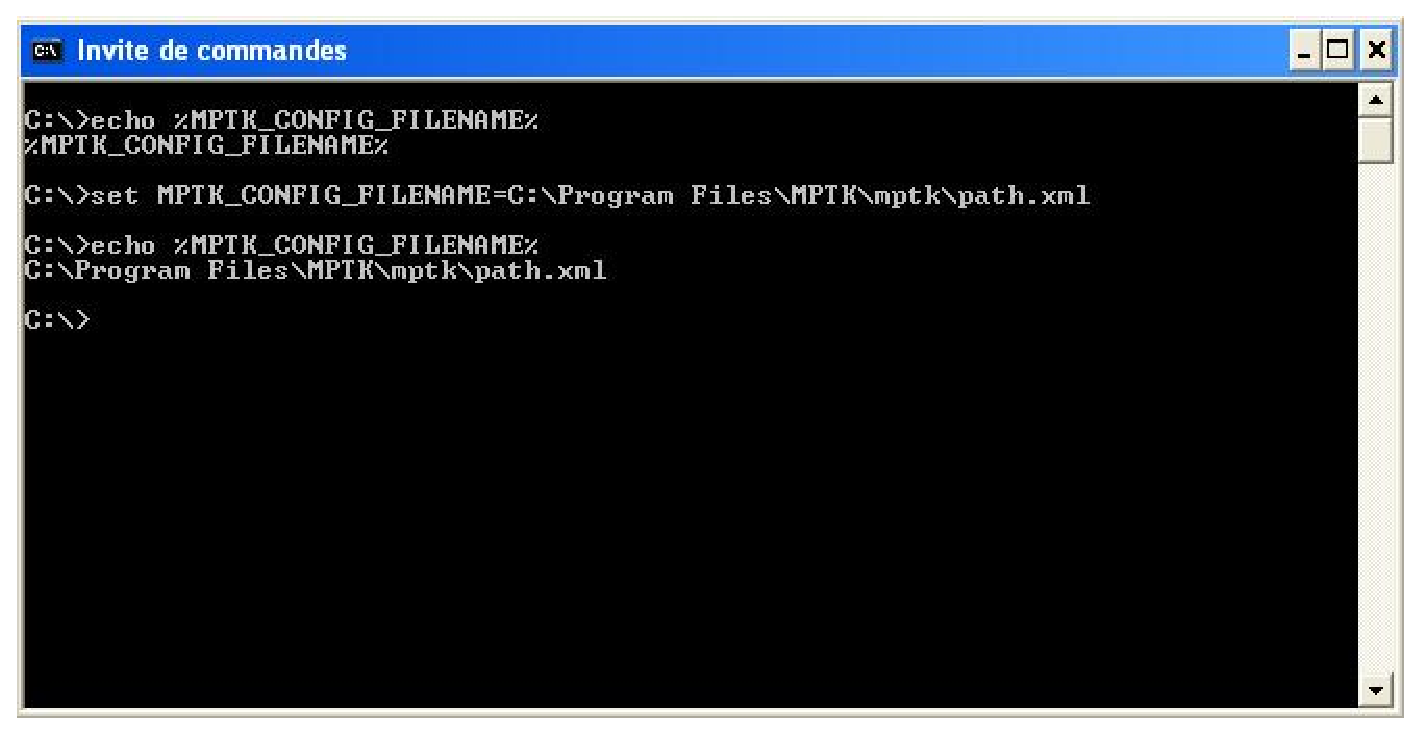
\includegraphics[width = 7cm, height=3cm]{Images/CommandPrompt.eps}
		\textit{\caption{\label{CommandPrompt} Filled command prompt}}
	\end{center}
\end{figure}

% Section 2.3.2 : Permanent path configuration

\subsection{Permanent path configuration}
 
\noindent Here is the way to permanently configure the \begin{footnotesize}MPTK\_CONFIG\_FILENAME\end{footnotesize} environment variable
\begin{my_itemize}
	\item Check if the environment variable is correctly set with : echo \begin{footnotesize}\%MPTK\_CONFIG\_FILENAME\%\end{footnotesize}
	\item Open the environment variable configuration panel situated under  :
	\begin{my_itemize}
		\item Start $\mapsto$ Config panel $\mapsto$ System $\mapsto$ Advanced $\mapsto$ Environment variables
	\end{my_itemize}
	\item Add a new user variable with :
	\begin{my_itemize}
		\item Name : \begin{footnotesize}MPTK\_CONFIG\_FILENAME\end{footnotesize}
		\item Value : \emph{path\_to\_MPTK/mptk/path.xml}
	\end{my_itemize}
\end{my_itemize}

\begin{figure}[H]
   	 \begin{center}
		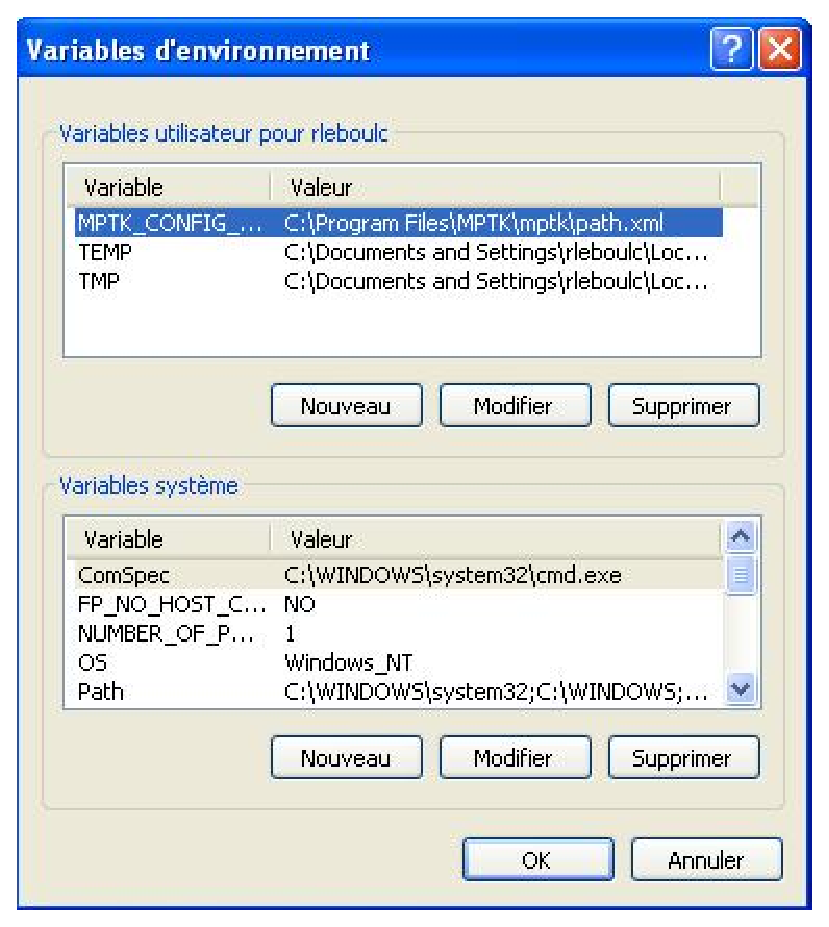
\includegraphics[width = 5cm, height=4cm]{Images/EnvironmentConfiguration.eps}
		\textit{\caption{\label{EnvironmentConfiguration} Environment variable configuration}}
	\end{center}
\end{figure}

% Section 2.3.2 : Matlab path configuration

\subsection{Matlab path configuration}

When launching Matlab, the user needs to configure Matlab to work with MPTK:
\begin{my_itemize}
	\item Configure the working path either by: 
	\begin{my_itemize}
		\item Selecting the current folder as \textcolor[rgb]{0.4,0.4,0.4}{``path\_to\_MPTK/mptk/matlab''}
		\item Adding the working path using \textcolor[rgb]{0.4,0.4,0.4}{addpath(``path\_to\_MPTK/mptk/matlab'')}
	\end{my_itemize}
\end{my_itemize}
